% Figure 1: all 44 DEPs by category. Compile with pdflatex, then
%   pdftoppm -png -r 200 -singlefile dep_sources.pdf dep_sources
\documentclass[border=12pt]{standalone}
\usepackage{lmodern}
\usepackage[T1]{fontenc}
\usepackage{tikz}
\usepackage{enumitem}
\usetikzlibrary{positioning,fit}

\definecolor{symb}{HTML}{D9D2E9}
\definecolor{reli}{HTML}{CFE2F3}
\definecolor{citi}{HTML}{D9EAD3}
\definecolor{bure}{HTML}{F4CCCC}
\definecolor{abro}{HTML}{E6A8EE}
\definecolor{netw}{HTML}{FFF2CC}
\definecolor{info}{HTML}{FFD966}
\definecolor{adva}{HTML}{FCCBAE}

% \depbox{name}{color}{title}{items}
\newcommand{\depbox}[4]{%
  \node[draw, fill=#2, anchor=north, minimum width=3.9cm, text width=3.7cm, minimum height=0.8cm, align=center, font=\bfseries\small, inner sep=4pt] (#1h) at (0,0) {#3};
  \node[draw, below=0pt of #1h, text width=3.7cm, minimum width=3.9cm, align=left, inner sep=4pt, font=\small] (#1) {%
    \begin{enumerate}[leftmargin=*, label=\arabic*., nosep]#4\end{enumerate}};
}

\begin{document}
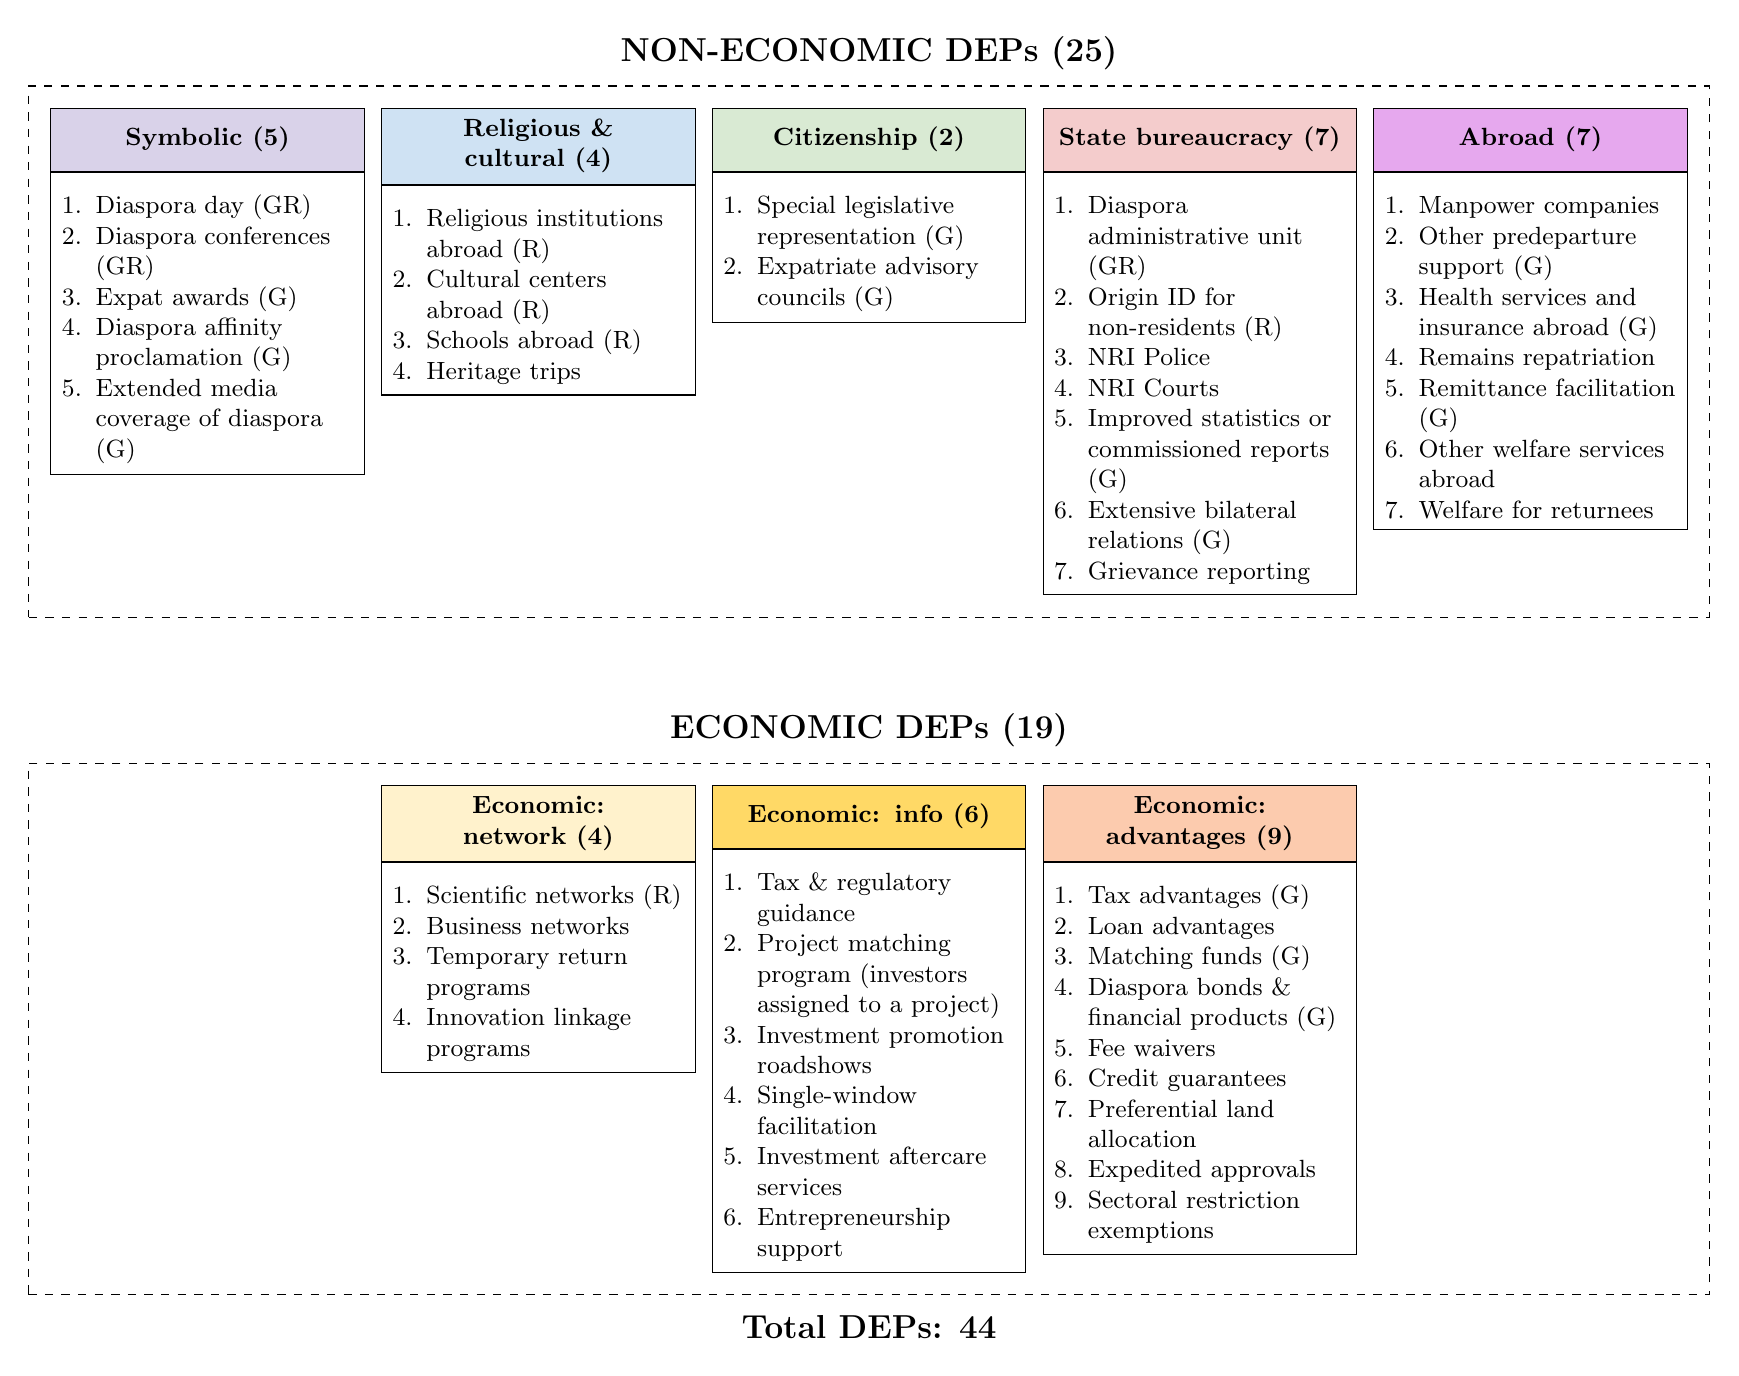
\begin{tikzpicture}
  % Non-economic row
  \begin{scope}[local bounding box=noneco]
    \begin{scope}[xshift=0cm]\depbox{a}{symb}{Symbolic (5)}{%
      \item Diaspora day (GR)
      \item Diaspora conferences (GR)
      \item Expat awards (G)
      \item Diaspora affinity proclamation (G)
      \item Extended media coverage of diaspora (G)}\end{scope}
    \begin{scope}[xshift=4.2cm]\depbox{b}{reli}{Religious \& cultural (4)}{%
      \item Religious institutions abroad (R)
      \item Cultural centers abroad (R)
      \item Schools abroad (R)
      \item Heritage trips}\end{scope}
    \begin{scope}[xshift=8.4cm]\depbox{c}{citi}{Citizenship (2)}{%
      \item Special legislative representation (G)
      \item Expatriate advisory councils (G)}\end{scope}
    \begin{scope}[xshift=12.6cm]\depbox{d}{bure}{State bureaucracy (7)}{%
      \item Diaspora administrative unit (GR)
      \item Origin ID for non-residents (R)
      \item NRI Police
      \item NRI Courts
      \item Improved statistics or commissioned reports (G)
      \item Extensive bilateral relations (G)
      \item Grievance reporting}\end{scope}
    \begin{scope}[xshift=16.8cm]\depbox{e}{abro}{Abroad (7)}{%
      \item Manpower companies
      \item Other predeparture support (G)
      \item Health services and insurance abroad (G)
      \item Remains repatriation
      \item Remittance facilitation (G)
      \item Other welfare services abroad
      \item Welfare for returnees}\end{scope}
  \end{scope}
  \node[draw, dashed, fit=(noneco), inner sep=8pt] (nebox) {};
  \node[above=2pt of nebox, font=\bfseries\large] {NON-ECONOMIC DEPs (25)};

  % Economic row
  \begin{scope}[yshift=-8.6cm, local bounding box=eco]
    \begin{scope}[xshift=4.2cm]\depbox{f}{netw}{Economic: network (4)}{%
      \item Scientific networks (R)
      \item Business networks
      \item Temporary return programs
      \item Innovation linkage programs}\end{scope}
    \begin{scope}[xshift=8.4cm]\depbox{g}{info}{Economic: info (6)}{%
      \item Tax \& regulatory guidance
      \item Project matching program (investors assigned to a project)
      \item Investment promotion roadshows
      \item Single-window facilitation
      \item Investment aftercare services
      \item Entrepreneurship support}\end{scope}
    \begin{scope}[xshift=12.6cm]\depbox{h}{adva}{Economic: \mbox{advantages} (9)}{%
      \item Tax advantages (G)
      \item Loan advantages
      \item Matching funds (G)
      \item Diaspora bonds \& financial products (G)
      \item Fee waivers
      \item Credit guarantees
      \item Preferential land allocation
      \item Expedited approvals
      \item Sectoral restriction exemptions}\end{scope}
  \end{scope}
  \path ([yshift=8pt]nebox.west |- eco.north) coordinate (ecl) ([yshift=-8pt]nebox.east |- eco.south) coordinate (ecr);
  \node[draw, dashed, fit=(ecl)(ecr), inner sep=0pt] (ebox) {};
  \node[above=2pt of ebox, font=\bfseries\large] {ECONOMIC DEPs (19)};
  \node[below=4pt of ebox, font=\bfseries\large] {Total DEPs: 44};
\end{tikzpicture}
\end{document}
